\documentclass[letterpaper,10pt]{article}
% use UTF8 encoding
\usepackage[utf8]{inputenc}
% use KoTeX package for Korean 
\usepackage[english]{babel}
\usepackage{multirow}
\usepackage{array}
\usepackage[dvipsnames]{xcolor}
\usepackage{kotex}
\usepackage{adjustbox}
\usepackage{tabularx} % extra features for tabular environment
\usepackage{amsmath}  % improve math presentation
\usepackage{amssymb}
\usepackage{graphicx} % takes care of graphic including machinery
\usepackage[margin=1in,letterpaper]{geometry} % decreases margins
\usepackage{cite} % takes care of citations
\usepackage[final]{hyperref} % adds hyper links inside the generated pdf file
\usepackage{minted}
\hypersetup{
	colorlinks=true,       % false: boxed links; true: colored links
	linkcolor=blue,        % color of internal links
	citecolor=blue,        % color of links to bibliography
	filecolor=magenta,     % color of file links
	urlcolor=blue         
}
\usepackage{blindtext}
%++++++++++++++++++++++++++++++++++++++++


\setlength{\parskip}{1.0em}
\renewcommand{\baselinestretch}{1.25}
\begin{document}
	
	\title{4. PyTorch Exercise}
	\author{2019920017 컴퓨터과학부 김정현}
	\date{2021/11/23까지}
	\maketitle
	
	\section{제출물에 대한 설명}
	
	이 과제에 대한 제출물은 이 보고서(report.pdf)를 포함하여 총 3개의 파일로 이루어져 있다. 각각에 대한 설명은 아래와 같다.
	
	\begin{enumerate}
		\item \textbf{report.pdf}: PyTorch를 이용하여 진행한 실험 결과를 정리하고, 이를 이용하여 Exercise의 각 물음에 답한다.
		
		\item \textbf{model-redefinition.ipynb}: 수업에서 다룬 PyTorch 코드에서 새로운 모델 정의($w_2 \times t_u^2 + w_1 \times t_u + b$)를 적용한 Jupyter 파일이다. \textbf{Exercise의 a, b번 물음에 답하기 위해 인용되며}, 어느 부분이 수정되었고, 어느 부분이 수정되지 않았는지를 확인할 수 있다.
		
		\item \textbf{experiments-to-compare.ipynb}: 기존의 모델($w \times t_u + b$)과 새로운 모델($w_2 \times t_u^2 + w_1 \times t_u + b$) 간의 성능 차이를 측정하기 위한 실험 과정을 정의한 Jupyter 파일이다. \textbf{Exercise의 c, d번 물음에 답하기 위해 인용되며}, 두 모델의 Loss 그래프에는 어떤 차이가 있는지, 평균적으로 어떤 모델이 더 높은 일반화 성능을 보이는지 확인한다.
	\end{enumerate}
	
	
	\section{질문에 대한 답안}
	
	\subsection{What parts of the training loop, and so on, need to change to accommodate this redefinition?}
	
	모델을 $w_2 \times t_u^2 + w_1 \times t_u + b$와 같이 새로 정의하기 위해서는 원래 코드에서 두 곳이 수정되어야 하는데, 이는 다음과 같다.
	
	\begin{enumerate}
		\item \textbf{model 함수의 인자와 구현}\\
		기존의 모델은 파라미터가 Bias를 포함하여 2개 뿐이었으나, 새로운 정의에서는 $w_1, w_2, b$로 총 3개가 존재하므로, 인자 역시 1개의 입력 스칼라와 3개의 파라미터를 받도록 수정해야 한다.\\
		그리고 $w_2 \times t_u^2 + w_1 \times t_u + b$ 식과 같이 결과를 계산하도록 구현을 수정하는 것이 필요하다.
		\begin{minted}
			[
			frame=lines,
			framesep=2mm,
			baselinestretch=1.2,
			fontsize=\footnotesize,
			linenos
			]
			{python3}
def model(t_u, w1, w2, b):
	return (w2 * t_u ** 2) + (w1 * t_u) + b
		\end{minted}
		
		\item \textbf{params 변수의 차원 수}\\
		새로운 모델에서는 3개의 파라미터를 사용하므로, \verb|training_loop| 함수에 전달되는 params는 3차원이 되어야 한다. 초기 파라미터의 값은 임의로 설정할 수 있으므로 아래 코드에서는 $(1, 0, 0)$으로 값을 설정하였다.
		\begin{minted}
			[
			frame=lines,
			framesep=2mm,
			baselinestretch=1.2,
			fontsize=\footnotesize,
			linenos
			]
			{python3}
params = torch.tensor([1.0, 0.0, 0.0], requires_grad=True)
		\end{minted}
		
	\end{enumerate}
	
	\subsection{What parts are agnostic to swapping out the model?}

	이전 질문에서 답변한 두 곳을 제외하면 그 외의 코드는 문제없이 재활용할 수 있다.
	
	이는 \verb|loss_fn|, \verb|training_loop| 등의 핵심적인 함수들이 모델에 종속적으로 구현된 것이 아니라 임의의 \verb|model| 함수에 대하여 동일한 과정으로 수행되도록 설계되었기 때문이다.
	
	비슷하게, 기존에 사용하던 데이터 셋이나 Optimizer도 문제없이 이용할 수 있는데, 이는 PyTorch 라이브러리가 임의의 Tensor에 대하여 동일하게 autograd를 지원하기 때문이다.

	\subsection{Is the resulting loss higher or lower after training?}
	
	Training data에 대한 Loss 값은 새로 정의된 모델이 더 작았으나, Validation data에 대한 Loss 값은 기존의 모델이 더 작았다. 아래 표와 그림은 두 모델을 학습시켰을 때 나타난 Loss 값을 나타낸 것이다.
	
	\begin{figure}[h]
		\centering
		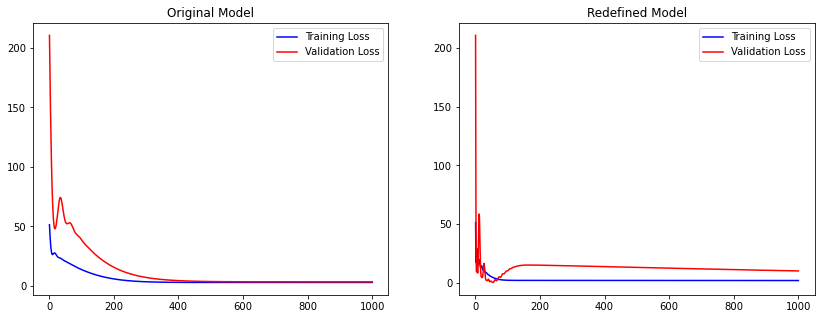
\includegraphics[width=\linewidth]{images/loss-cmp.png}
		\caption{두 모델의 Training, Validation Loss를 그린 그래프.}
	\end{figure}
	
	\begin{table}[]
		\centering
		\begin{tabular}{c|ll|ll}
			\multicolumn{1}{l|}{} & \multicolumn{2}{c|}{Original} & \multicolumn{2}{c}{Redefined} \\ \hline
			Epochs                & Training     & Validation     & Training     & Validation     \\ \hline
			1                     & 51.4150      & 210.6365       & 51.4150      & 210.6365       \\ \hline
			2                     & 45.8208      & 189.5128       & 23.1888      & 75.3991        \\ \hline
			3                     & 40.9619      & 169.7757       & 17.3617      & 15.7157        \\ \hline
			500                   & 2.9175       & 3.6702         & 2.1791       & 13.3067        \\ \hline
			1000                  & 2.9111       & 3.3966         & 2.1270       & 10.2992        \\ \hline
		\end{tabular}
		\caption{두 모델에 대하여 1,000 epochs 만큼 학습시켰을 때 나타난 Loss 값.}
	\end{table}
	
	새로 정의된 모델의 Training Loss 값이 기존 모델의 값보다 가파르게 하락하며, 최종 Training Loss 역시 새로 정의된 모델이 더 작다. Validation Loss는 초기에 새로 정의된 모델이 더 빠르게 작아지지만 가장 마지막에는 새로 정의된 모델이 10.3, 기존의 모델이 3.3으로 기존의 모델이 더 높은 일반화 성능을 보인다. 
	
	\subsection{Is the actual result better or worse?}
	
	결과적으로, \textbf{새로 정의된 모델은 기존의 모델보다 나쁜 일반화 성능을 보인다.} 다시 말하면, Overfitting이 쉽게 발생하여 Training Loss에 비해 Validation Loss가 상대적으로 매우 크다는 것이다.
	
	기존의 모델과 새로운 모델에 대하여 같은 방법으로 20회 동일한 실험을 반복하면서 Validation Loss가 Training Loss 보다 몇 퍼센트나 높은지 측정한 결과, \textbf{기존의 모델은 116.66\%, 새로운 모델은 484.21\%}를 나타내었다. 이러한 결과는 새로운 모델이 Overfitting에 훨씬 취약하다는 사실을 시사한다.
	
	\begin{minted}
		[
		frame=lines,
		framesep=2mm,
		baselinestretch=1.2,
		fontsize=\footnotesize,
		linenos
		]
		{text}
After 20 experiments...
	Original: Validation loss is 116.675915735631% greater than training loss.
	Redefined: Validation loss is 484.2144294637739% greater than training loss.
	\end{minted}

	그런데, Figure 1의 그래프를 확인해보면 앞서 언급한 것 처럼 새로운 모델은 Overfitting이 발생한 것을 쉽게 확인할 수 있으나, 학습의 초기에 Validation Loss와 Training Loss가 모두 낮은 순간이 존재함을 확인할 수 있다. \textbf{만약 Overfitting이 발생하기 전, 두 Loss 값이 함께 낮은 순간에 맞춰 학습을 종료할 수 있다면, 기존의 모델보다 더 좋은 성능을 얻을 수 있을 것이다.}
	
\end{document}
